
\chapter{INTRODUCTION}

\section{Onion Routing}

As the prevalence of the Internet and other communication has grown, so too has the development and usage of privacy-enhancing systems. These are tools and protocols that provide privacy by obfuscating the link between a user's identification or location and their communications. Privacy is not achieved in traditional Internet connections because SSL/TLS encryption cannot hide IP and TCP headers, which must be exposed to allow routing between two parties; eavesdroppers can easily break user privacy by monitoring these headers. A closely related property is anonymity -- a part of privacy where user activities cannot be tracked and their communications are indistinguishable from others. Tools that provide these systems hold a user's identity in confidence, and privacy and anonymity are often provided together. Following a general distrust of unsecured Internet communications and in light of the 2013-current revelations by Edward Snowden of Internet mass-surveillance by the NSA, GCHQ, and other members of the Five Eyes, users have increasingly turned to these tools for their own protection. Privacy-enhancing and anonymity tools may also be used by the military, researchers working in sensitive topics, journalists, law enforcement running tip lines, activists and whistleblowers, or individuals in countries with Internet censorship. These users may turn to proxies or VPNs, but these tools often track their users for liability reasons and thus rarely provide anonymity. Furthermore, they can easily voluntarily or be forced to break confidence to destroy user privacy. More complex tools are needed for a stronger guarantee of privacy and anonymity.

Today, most anonymity tools descend from mixnets, an early anonymity system invented by David Chaum in 1981.\cite{chaum2003untraceable} In a mixnet, user messages are transmitted to one or more mixes, who each partially decrypt, scramble, delay, and retransmit the messages to other mixes or to the final destination. This enhances privacy by heavily obscuring the correlation between the origin, destination, and contents of the messages. Mixnets have inspired the development of many varied mixnet-like protocols and have generated significant literature within the field of network security.\cite{edman2009anonymity}\cite{syverson2011peel}

Mixnet descendants can generally be classified into two distinct categories: high-latency and low-latency systems. High-latency networks typically delay traffic packets and are notable for their greater resistance to global adversaries who monitor communication entering and exiting the network. However, high-latency networks, due to their slow speed, are typically not suitable for common Internet activities such as web browsing, instant messaging, or the prompt transmission of email. Low-latency networks, by contrast, do not delay packets and are thus more suited for these activities, but they are more vulnerable to timing attacks from global adversaries.\cite{dingledine2004tor} In this work, we detail and introduce new functionality within low-latency protocols.

Onion routing is a technique for enhancing privacy of TCP-based communication across a network and is the most popular low-latency descendant of mixnets in use today. It was first designed by the U.S. Naval Research Laboratory in 1997 for military applications\cite{syverson1997anonymous}\cite{reed1998anonymous} but has since seen widespread usage. In onion routing with public key infrastructure (PKI), a user selects a set network nodes, typically called \emph{onion routers} and together a \emph{circuit}, and encrypts the message with the public key of each router. Each encryption layer contains the next destination for the message -- the last layer contains the message's final destination. As the \emph{cell} containing the message travels through the network, each of these onion routers in turn decrypt their encryption layer like an onion, exposing their share of the routing information. The final recipient receives the message from the last router, but is never exposed to the message's source.\cite{syverson2011peel} The sender therefore has privacy because the recipient does not know the sender's location, and the sender has anonymity if no identifiable or distinguishing information is included in their message.

\begin{figure}[htbp]
	\centering
	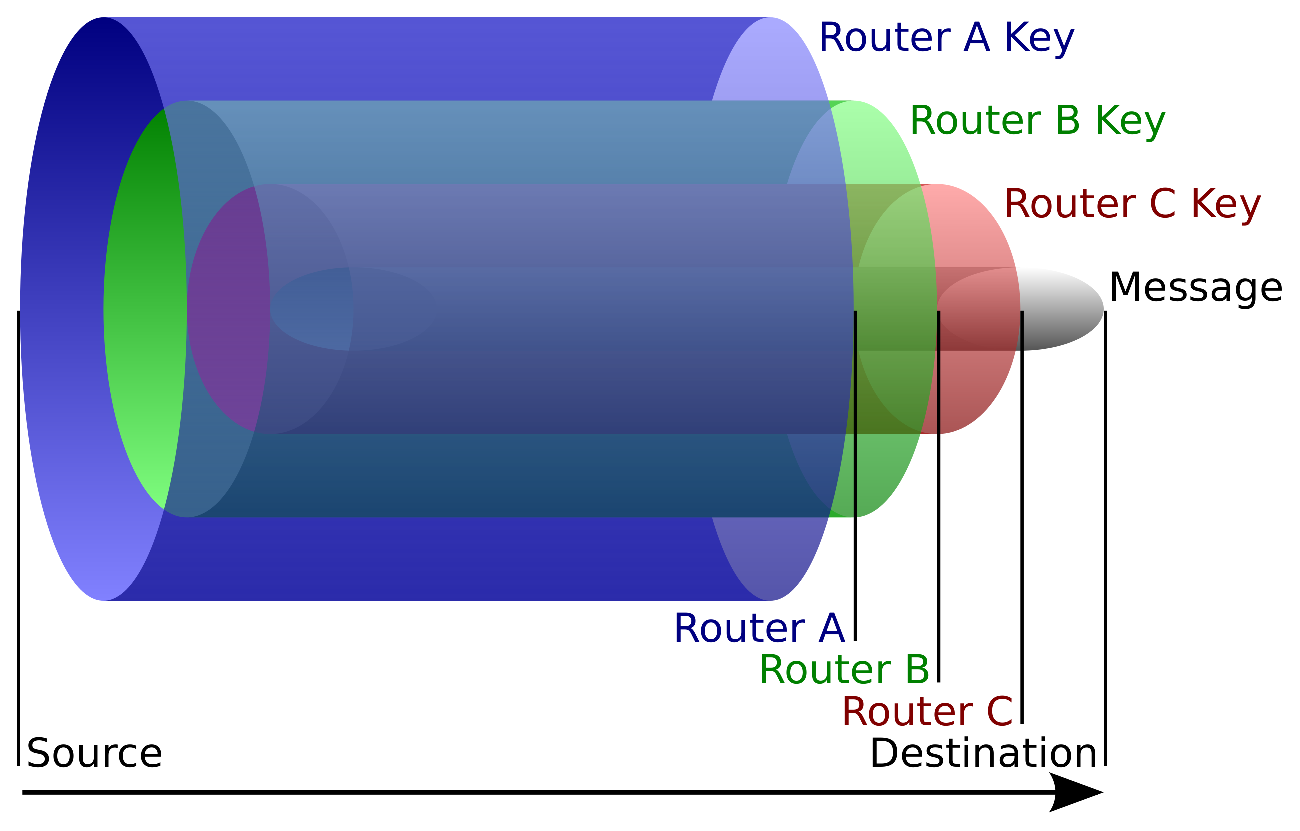
\includegraphics[width=0.5\textwidth]{images/onion-diagram.eps}
	\caption{An example cell and message encryption in an onion routing scheme. Each router ``peals'' off its respective layer of encryption; the final router exposes the final destination.}
\end{figure}

The first generation of onion routing used circuits fixed to a length of five, assumed a static network topology, and most notably, introduced the ability to mate two circuits at a common node or server. This last capability enabled broader anonymity where the circuit users were anonymous to each other and to the common server, a capability that was adopted and refined by later generation onion routers. Second generation introduced variable-length circuits, multiplexing of all user traffic over circuits, exit policies for the final router, and assumed a dynamic network by routing updates throughout the network. A client, Alice, in second-generation onion routers also distributed symmetric keys through the cell layers. If routers remember the destinations for each message they received, the recipient Bob can send his reply backwards through the circuit and each router re-encrypts the reply with their symmetric key. Alice unwraps all the layers, exposing the Bob's reply. The transition from public-key cryptography to symmetric-key encryption significantly reduced the CPU load on onion routers and enabled them to transfer more packets in the same amount of time. However, while influential, first and second generation onion routing networks have fallen out of use in favor of third-generation systems.\cite{syverson2011peel}

\section{Tor}

Tor is a third-generation onion routing system. It was invented in 2002 by Roger Dingledine, Nick Mathewson, and Paul Syverson of the Free Haven Project and the U.S. Naval Research Laboratory\cite{dingledine2004tor} and is the most popular onion router in use today. Tor inherited many of the concepts pioneered by earlier onion routers and implemented several key changes:\cite{syverson2011peel}\cite{dingledine2004tor}

\begin{itemize}
	\item \textbf{Perfect forward secrecy:} Rather than distributing keys via onion layers, Tor clients negotiate a TLS Diffie-Hellman-Merkle ephemeral key exchange with each of the routers in turn, extending the circuit one node at a time. These keys are then purged when the circuit is torn down; this achieves perfect forward secrecy, a property that ensures that the symmetric encryption keys will not be revealed if long-term public keys are later compromised.
	\item \textbf{Circuit isolation:} Second-generation onion routers mixed cells from different circuits in realtime, but later research could not justify this as an effective defence against an active adversary.\cite{syverson2011peel} Tor abandoned this in favor of isolating circuits from each other inside the network. Tor circuits are used for up to 10 minutes or whenever the user chooses to rotate to a fresh circuit.
	\item \textbf{Three-hop circuits:} Previous onion routers used long circuits to provide heavy traffic mixing. Tor removed mixing and fell back to using short circuits of minimal length. With three relays involved in each circuit, the first node (the \emph{guard}) is exposed to the user's IP address. The middle router passes onion cells between the guard and the final router (the \emph{exit}) and its encryption layer exposes it to neither the user's IP nor its traffic. The exit processes user traffic, but is unaware of the origin of the requests. While the choice of middle and exits can be routers can be safely random, the guard nodes must be chosen once and then consistently used to avoid a large cumulative chance of leaking the user's IP to an attacker. This is of particular importance for circuits from hidden services.\cite{bauer2007low}\cite{overlier2006locating}
	\item \textbf{Standardized to SOCKS proxy:} Tor simplified the multiplexing pipeline by transitioning from application-level proxies (HTTP, FTP, email, etc) to a TCP-level SOCKS proxy, which multiplexed user traffic and DNS requests through the onion circuit regardless of any higher protocol. The disadvantage to this approach is that Tor's client software has less capability to cache data and strip identifiable information out of a protocol. The countermeasure was the Tor Browser, a fork of Mozilla's open-source Firefox with a focus on security and privacy. To reduce the risks of users breaking their privacy through Javascript, it ships with the NoScript extension which blocks all web scripts not explicitly whitelisted. The browser also forces all web traffic, including DNS requests, through the Tor SOCKS proxy, provides a Windows-Firefox user agent regardless of the native platform, and includes many additional security and privacy enhancements not included in native Firefox. The browser also utilizes the EFF's HTTPS Everywhere extension to re-write HTTP web requests into HTTPS whenever possible; when this happens the Tor cell contains an additional inner encryption layer.
	\item \textbf{Directory servers:} Tor introduced a set of trusted directory servers to distribute network information and the public keys of onion routers. Onion routers mirror the digitally signed network information from the directories, distributing the load. This simplified approach is more flexible and scales faster than the previous flooding approach, but relies on the trust of central directory authorities. Tor ensures that each directory is independently maintained in multiple locations and jurisdictions, reducing the likelihood of an attacker compromising all of them.\cite{syverson2011peel} We describe the contents and format of the network information published by the directories in section \ref{sec:ConsensusDocs}.
	\item \textbf{Dynamic rendezvous with hidden services:} In previous onion routers, circuits mated at a fixed common node and did not use perfect forward secrecy. Tor uses a distributed hashtable to record the location of the introduction node for a given hidden service. Following the initial handshake, the hidden service and the client then meet at a different onion router chosen by the client. This approach significantly increased the reliability of hidden services and distributed the communication load across multiple rendezvous points.\cite{dingledine2004tor} We provide additional details on the hidden service protocol in section \ref{sec:HiddenServices} and our motivation for addition hidden service infrastructure in section \ref{sec:Motivation}.
\end{itemize}

As of March 2015, Tor has 2.3 million daily users that together generate 65 Gbit/s of traffic. Tor's network consists of nine authority nodes and 6,600 onion routers in 83 countries.\cite{TorMetrics} In a 2012 Top Secret U.S. National Security Agency presentation leaked by Edward Snowden, Tor was recognized as the "the king of high secure, low latency Internet anonymity".\cite{landau2014highlights}\cite{plak2014anonymous} In 2014, BusinessWeek claimed that Tor was ``perhaps the most effective means of defeating the online surveillance efforts of intelligence agencies around the world.''\cite{TorBusinessWeek}

\subsection{Design}

Tor's design focuses on being easily deployable, flexible, and well-understood. Tor also places emphasis on usability in order to attract more users; more user activity translates to an increased difficulty of isolating and breaking the privacy of any single individual. Tor however does not manipulate any application-level protocols nor does it make any attempt to defend against global attackers. Instead, its threat model assumes that the capabilities of adversaries are limited to observing fractions of Tor traffic, that they can actively delay, delete, or manipulate traffic, that they may attempt to digitally fingerprint packets, that they may run onion routers themselves, and that they may compromise a fraction of other existing routers. Together, most of the assumptions may be broadly classified as traffic analysis attacks. Tor's final focus is defending against these types of attacks.\cite{dingledine2004tor}

\subsection{Circuit Construction}

\subsubsection{Overview}

Let Alice be a client who wishes to enhance her privacy by using Tor but does not run a Tor router herself. Her basic procedure for initializing her own circuit is as follows:

\begin{enumerate}
	\item Alice selects a Tor router $ R_{1} $ and establishes an encrypted connection to it.
	\item Alice selects a second router $ R_{2} $ and tells $ R_{1} $ to ensure that a TCP link is available to it. 
	\item Alice uses her link with $ R_{1} $ to establish an encrypted connection with $ R_{2} $.
	\item Alice selects an $ R_{3} $ and uses the $ Alice \leftrightarrow R_{1} \leftrightarrow R_{2} $ tunnel to tell $ R_{2} $ to connect to $ R_{3} $.
	\item Alice establish an encrypted connection with $ R_{3} $ over the $ Alice \leftrightarrow R_{1} \leftrightarrow R_{2} $ tunnel.
\end{enumerate}

Following the successful circuit construction, she can then send messages out of $ R_{3} $ through the $ Alice \leftrightarrow R_{1} \leftrightarrow R_{2} \leftrightarrow R_{3} $ tunnel.

As a defense against traffic analysis using packet size, Alice packs and pads circuit traffic into equally-sized Tor \emph{cells} of 512 bytes and changes $ R_{2} $ and $ R_{3} $ every 10 minutes.\cite{mccoy2008shining}

\emph{TODO: Tor chooses the guard carefully}

\subsubsection{TAP}

The Tor Authentication Protocol (TAP) is a critical piece of Tor networking infrastructure as it allows Alice to verify the authenticity of the onion routers that she selects for her circuit while still remaining anonymous herself. Namely it prevents active spoofing attacks, which if successful would deanonymize Alice and compromise her privacy.

First, TAP assumes that the following is established:

\begin{itemize}
	\item Alice has a reliable PKI that can securely distribute the identity, IP addresses, and public keys of all Tor routers. Tor accomplishes this through consensus documents from authority nodes, described in section \ref{sec:ConsensusDocs}.
	\item Let $ \mathcal{E}_{B} $ mean encryption and $ \mathcal{D}_{B} $ mean decryption under $ B $'s public-private keypair for some party $ B $.
	\item $ p $ is a prime such that $ q = \frac{q - 1}{2} $ is also prime and let $ g $ be a generator of the subgroup of $ \mathbb{Z}^{*}_{p} $ of order $ q $.
	\item Let $ R_{L} $ be a generator that returns uniformly random $ L $-bit values in the interval $ [1, \textrm{min}(q, 2 ^ L) - 1] $.
	\item Define $ f $ as SHA-1 which takes input from $ \mathbb{Z}_{p} $ and returns a $ L_{f} $-bit value.
\end{itemize}

Then TAP proceeds as:

\begin{enumerate}
	\item \label{item:First1}
		Alice selects a Tor router, $ R_{i} $.
	\item
		Alice generates $ x = R_{L} $ and computes $ s = g ^ x \bmod{p} $.
	\item
		Alice sends $ c = \mathcal{E}_{R_{i}}(s) $ to $ R_{i} $.
	\item
		$ R_{i} $ computes $ m = \mathcal{D}_{R_{i}}(c) $ and confirms that $ 1 < m < p - 1 $.
	\item
		$ R_{i} $ generates $ y = R_{L} $ and computes $ a = g ^ y \bmod{p} $ and $ b = f(m ^ y \bmod{p}) $.
	\item
		$ R_{i} $ sends $ (a, b) $ to Alice.
	\item
		Alice confirms that $ 1 < a < p - 1 $ and that $ b = f(a ^ x \bmod{p}) $.
	\item \label{item:Last1}
		If the assertions pass, then Alice has confirmed $ R_{i} $'s identity and now Alice and $ R_{i} $ can use $ a ^ x = m ^ y $ as a shared symmetric encryption key and encrypt messages under AES.
	\item 
		Alice repeats steps \ref{item:First1} -- \ref{item:Last1} until the circuit is of the desired length.
\end{enumerate}

Thus for each router in the circuit, Alice perform one public-key encryption and her half of a Diffie-Hellman-Merkle handshake, and each router in turn performs one private-key decryption and their half of a Diffie-Hellman-Merkle handshake. Under the assumptions that RSA is one way, AES remains unbroken, and $ f $ is strong and acts as a random oracle, an attacker has only a negligible chance of being able to impersonate $ R_{i} $ and read messages that she tunnels through the circuit.\cite{goldberg2006security}

\subsubsection{NTor}

In mid 2013, TAP was superseded by ``NTor'', a new protocol invented by Goldberg, Stebila, and Ustaoglu.\cite{goldberg2013anonymity} Compared to TAP, NTor requires less computational demand and uses stronger cryptographic primitives.

First,

\begin{itemize}
	\item Let $ H(x,t) $ be HMAC-SHA256, which accepts a message $ x $ and key $ t $ and returns a 32-byte output.
	\item Let $ K_{\mathit{gen}} $ yield $ a $ and $ A $, the private and public halves, respectively, of the Curve25519\cite{bernstein2006curve25519} keypair.
	\item Let each Tor router $ R_{j} $ generate $ a_{j},A_{j} = K_{\mathit{gen}} $ and publish $ A_{j} $ through the consensus document.
\end{itemize}

Then NTor proceeds as:

\begin{enumerate} % 216-ntor-handshake.txt
	\item \label{item:First2}
		Alice selects a Tor router, $ R_{i} $.
	\item
		Alice generates $ x_{i}, X_{i} = K_{\mathit{gen}} $.
	\item
		Alice sends $ X_{i} $ to $ R_{i} $.
	\item
		$ R_{i} $ receives $ X_{i} $ and computes $ y_{i}, Y_{i} = K_{\mathit{gen}} $.
	
\end{enumerate}

% --begin rewrite required

%\emph{This section is incomplete. Here I will describe the Tor Authentication Protocol which has since been extended to use ECDHE with ed25519 ECDSA:  and called NTor.\cite{goldberg2013anonymity} I will walk through this protocol.}

%\begin{figure}[htdp]
%	\begin{minipage}[b]{0.45\linewidth}
%		\centering
%		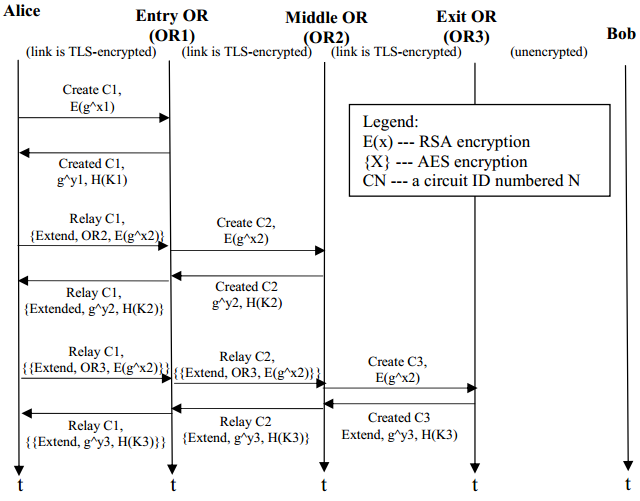
\includegraphics[width=\textwidth]{images/Tor/circuit-construction.png}
%		\caption{Anatomy of the construction of a Tor circuit.}
%		\label{fig:figure1}
%	\end{minipage}
%	\hspace{0.5cm}
%	\begin{minipage}[b]{0.45\linewidth}
%		\centering
%		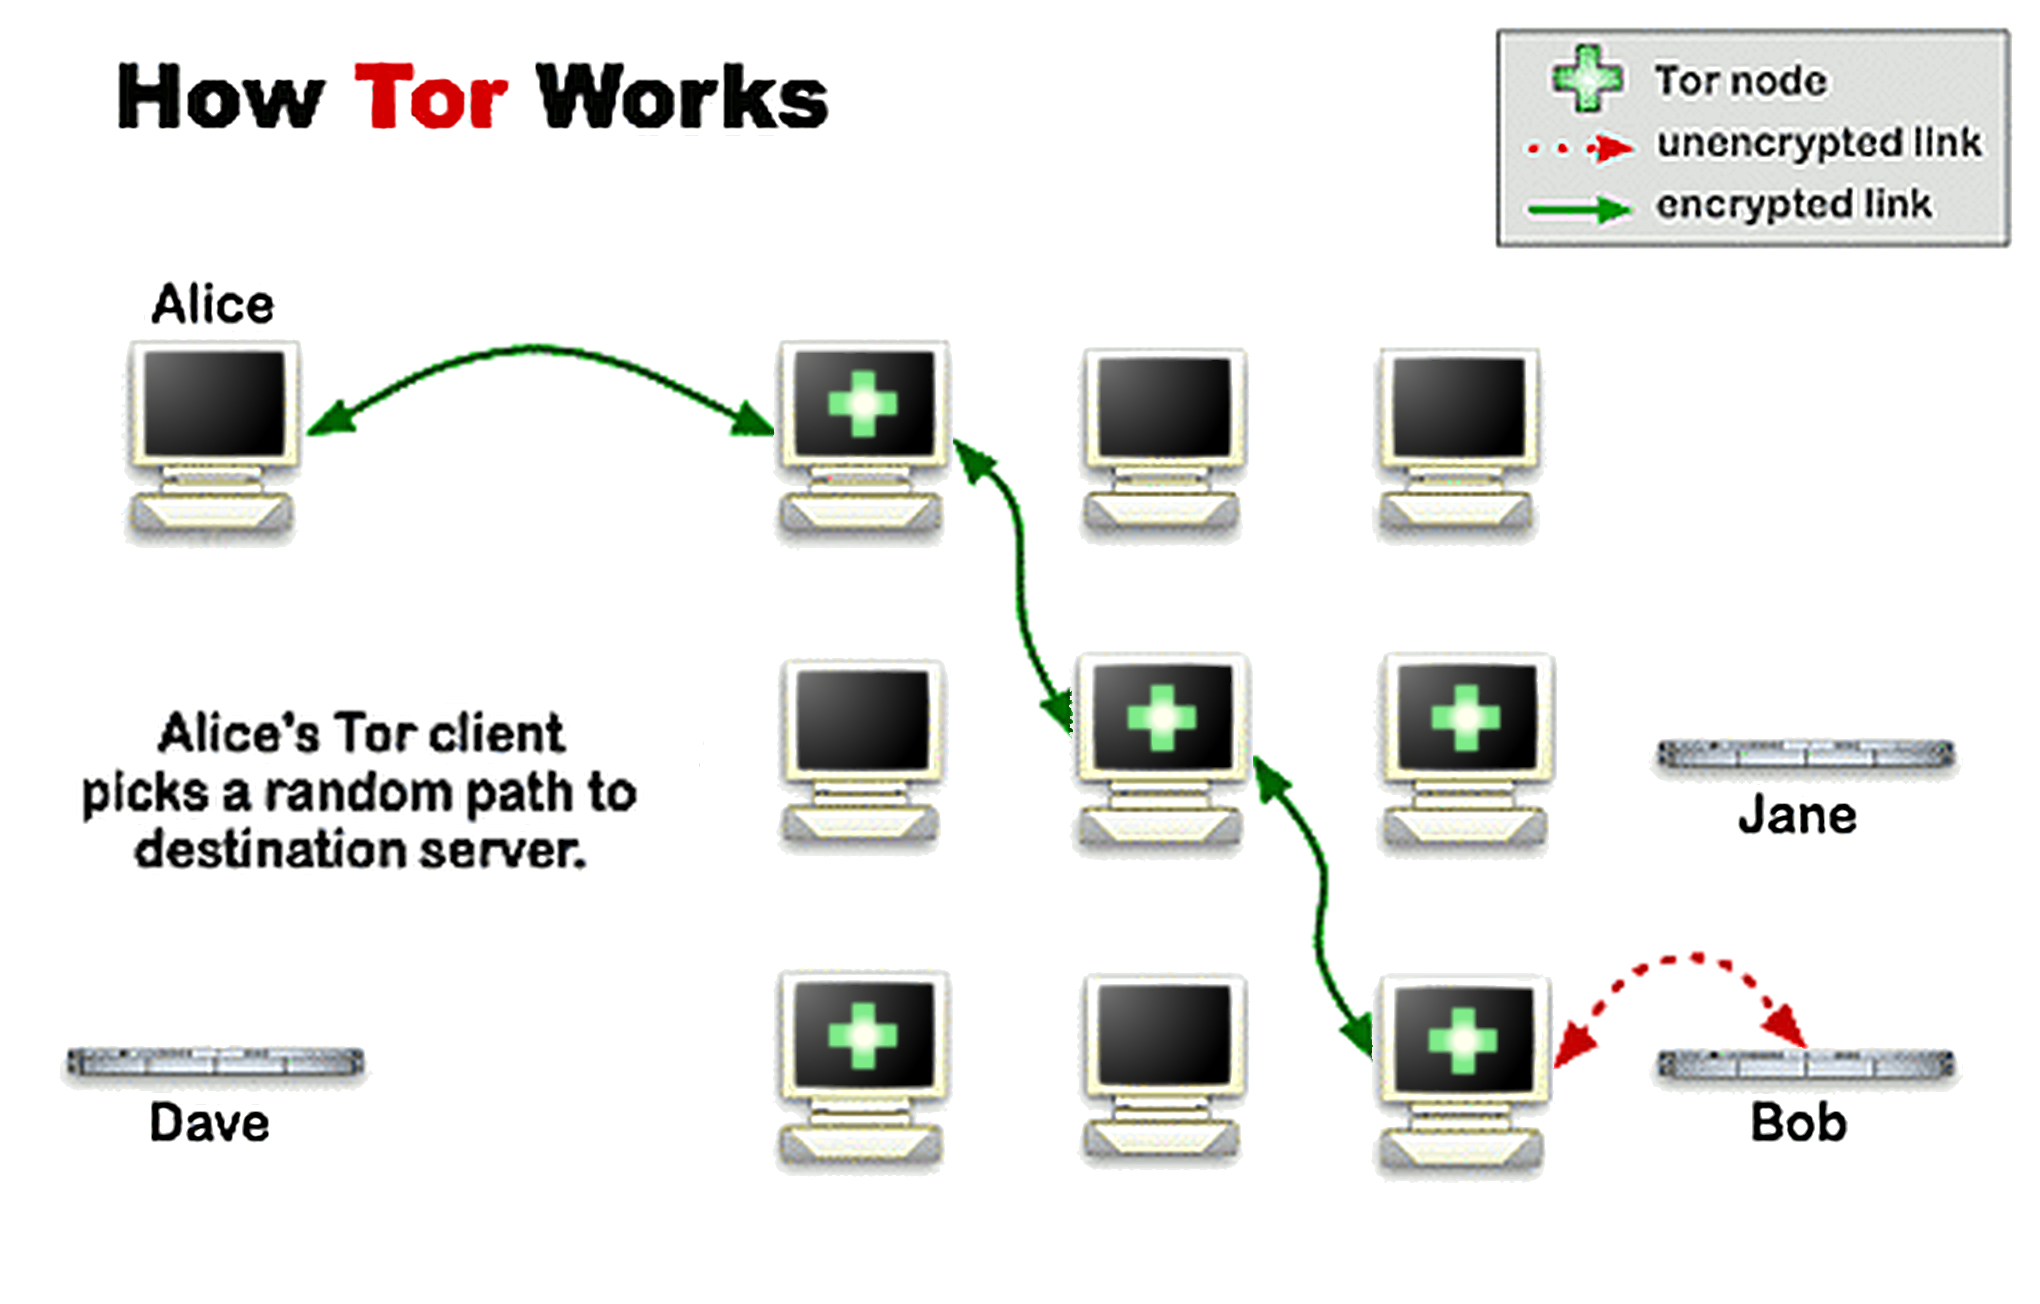
\includegraphics[width=\textwidth]{images/Tor/circuit-building-2-5.png}
%		\caption{A circuit through the Tor network.}
%		\label{fig:figure2}
%	\end{minipage}
%\end{figure}
%

%The client first establishes a TLS connection with the first relay, $R_{1}$, using the relay's public key. The client then performs an ECDHE key exchange to negotiate $K_{1}$ which is then used to generate two symmetric session keys: a forward key $K_{1,F}$ and a backwards key $K_{1,B}$. $K_{1,F}$ is used to encrypt all communication from the client to $R_{1}$ and $K_{1,B}$ is used for all replies from $R_{1}$ to the client. These keys are used conjunction with the symmetric cipher suite negotiated during the TLS handshake, thus forming an encrypted tunnel with perfect forward secrecy. Once this one-hop circuit has been created, the client then sends $R_{1}$ the RELAY\_EXTEND command, the address of $R_{2}$, and the client's half of the Diffie-Hellman-Merkle protocol using $K_{1,F}$. $R_{1}$ performs a TLS handshake with $R_{2}$ and uses $R_{2}$'s public key to send this half of the handshake to $R_{2}$, who replies with his second half of the handshake and a hash of $K_{2}$. $R_{1}$ then forwards this to the client under $R_{1,B}$ with the RELAY\_EXTENDED command to notify the client. The client generates $K_{1,F}$ and $K_{1,B}$ from $K_{2}$, and repeats the process for $R_{3}$,\cite{ling2013protocol} as shown in Figure 3. The TCP/IP connections remain open, so the returned information travels back up the circuit to the end user.



%\begin{figure}[htbp]
%	\centering
%	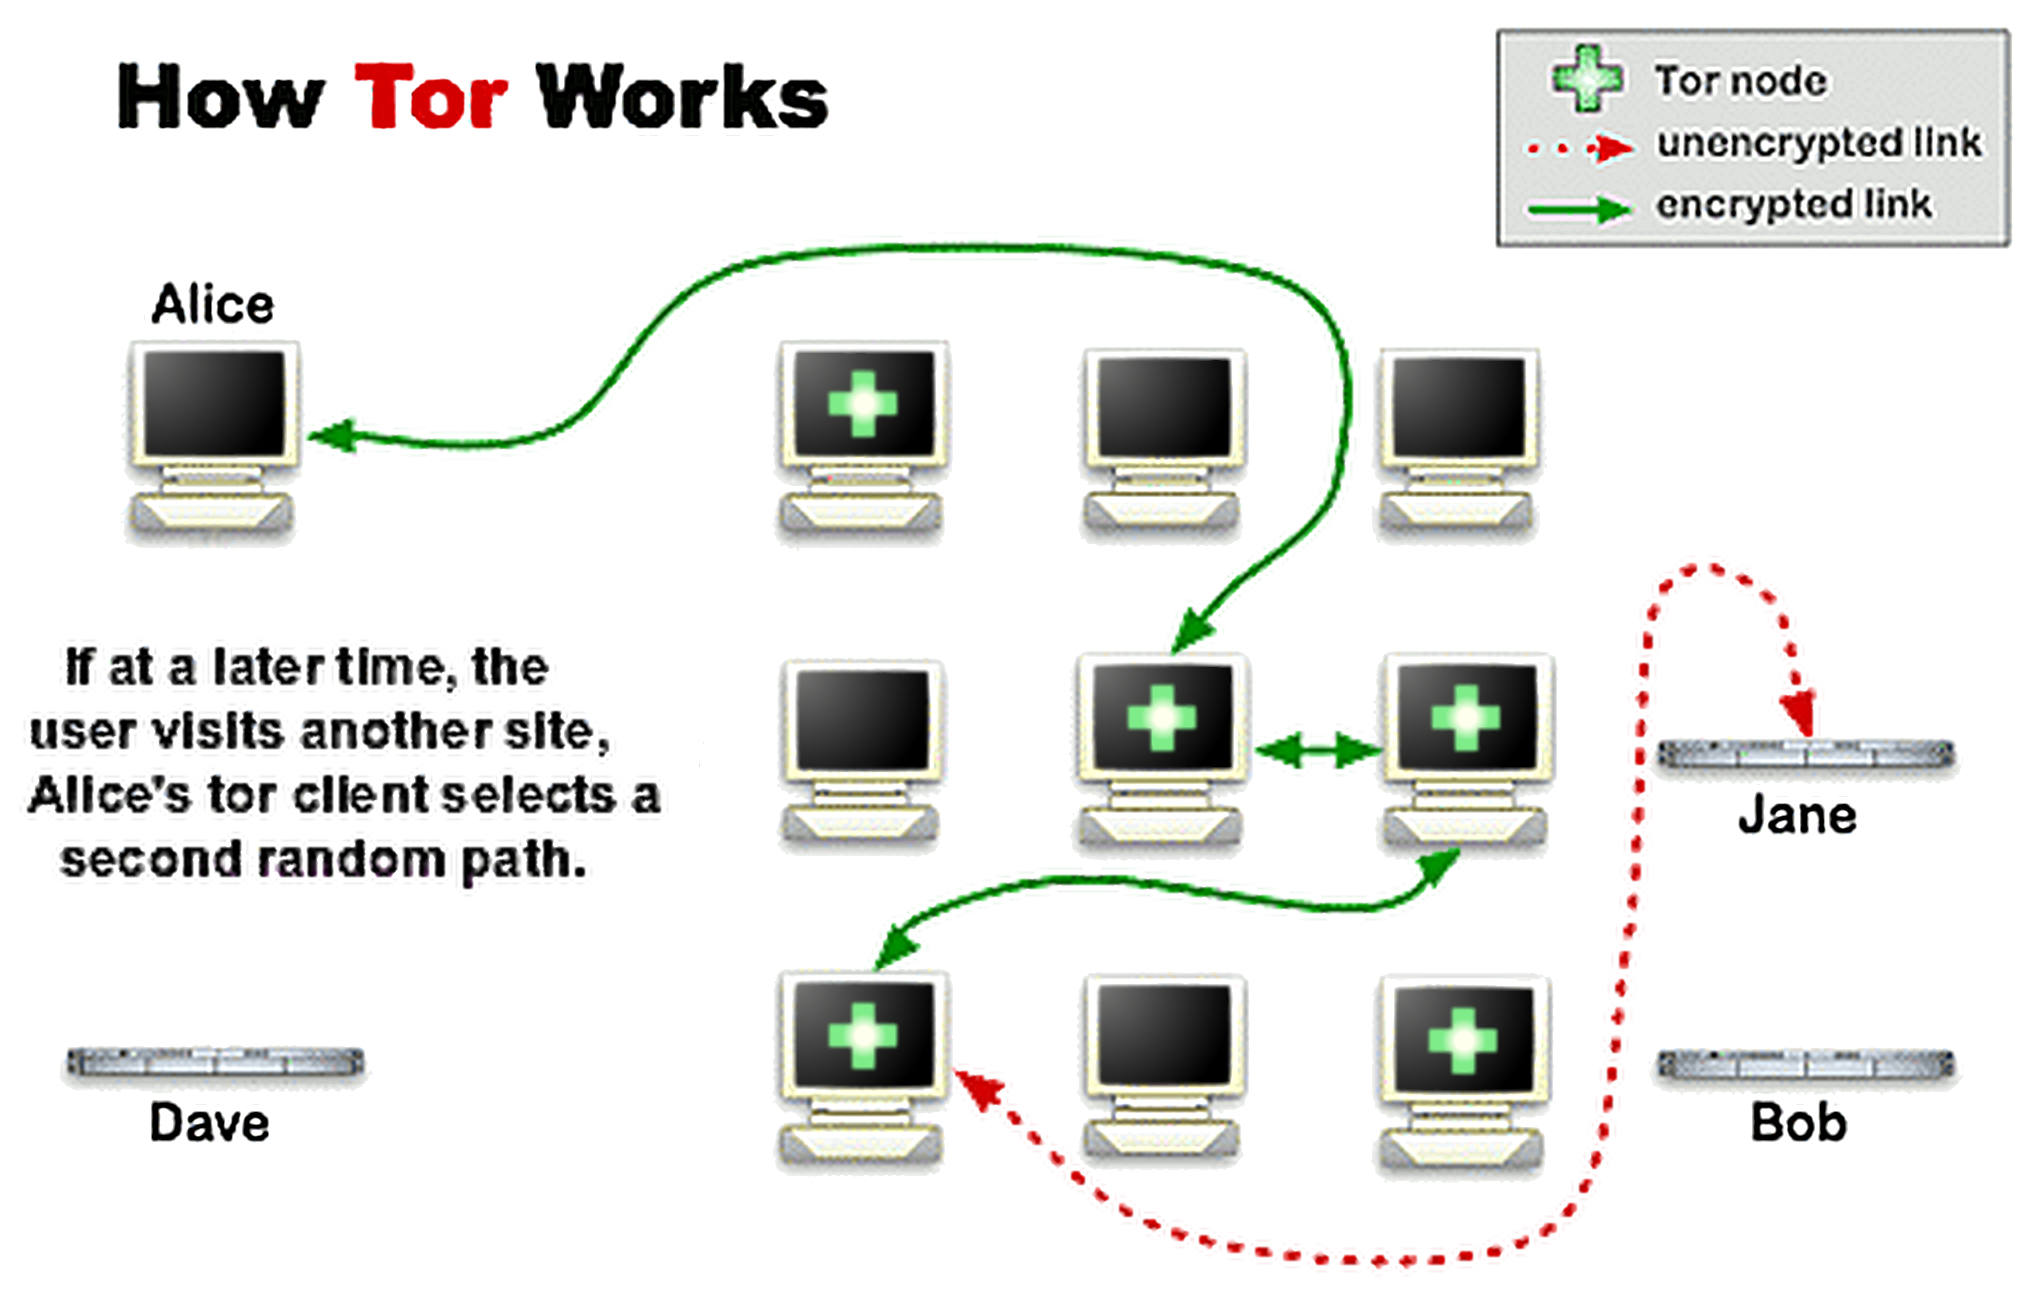
\includegraphics[width=0.6\textwidth]{images/Tor/circuit-change-1-4.png}
%	\caption{A Tor circuit is changed periodically, creating a new user identity.}
%\end{figure}
%
%% Although a different guard node is used here, in practice the choice of entry point is preserved for extended periods of time.
%
% If this happens, end-to-end encryption is complete and an outsider near the user would be faced with up to four layers of TLS encryption: $K_{1,F}(K_{2,F}(K_{3,F}(K_{server}(\textrm{client\ request}))))$ and likewise $K_{1,B}(K_{2,B}(K_{3,B}(K_{server}(\textrm{server\ reply}))))$ for the returning traffic, making traffic analysis very difficult.









\subsection{Consensus Documents}
\label{sec:ConsensusDocs}

The Tor network is maintained by nine authority nodes, who each vote on the status of nodes and together hourly publish a digitally signed consensus document containing IPs, ports, public keys, latest status, and capabilities of all nodes in the network. The document is then redistributed by other Tor nodes to clients, enabling access to the network. The document also allows clients to authenticate Tor nodes when constructing circuits, as well as allowing Tor nodes to authenticate one another. Since all parties have prior knowledge of the public keys of the authority nodes, the consensus document cannot be forged or modified without disrupting the digital signature.\cite{xin2009design}

\emph{Here I plan to detail the consensus documents that I will be using, since I use them in my Solution section.}

\subsection{Hidden Services}
\label{sec:HiddenServices}

Although Tor's primary and most popular use is for secure access to the traditional Internet, Tor also supports anonymous services, such as websites, marketplaces, or chatrooms. These are a part of the Dark Web and cannot be normally accessed outside the context of Tor. In contrast to Tor-anonymized web requests where the client is anonymous but the server is known, Tor hidden services provide bidirectional anonymity where both parties remain anonymous and never directly communicate with one another. This allows for a greater range of communication capabilities.\cite{nicolussi2011human}

Tor does not contain a DNS system for its websites; instead hidden service addresses are algorithmically generated by generating the SHA-1 hash of their public RSA key, truncating to 80 bits, and converting the remainder to base58. Ignoring the possibility of SHA-1 collisions, this builds a one-to-one relationship between a hidden service's public key and its address which can be confirmed without requiring any identifiable information or central authorities. The address is the appended with the .onion Top-Level Domain (TLD).

A hidden server, Bob, first builds Tor circuits to several random relays and enables them to act as \textit{introduction points} by giving them its public key, $ B_{K} $. He then then uploads his public key and the fingerprint identity of these nodes to a distributed hashtable inside the Tor network, signing the result. He then publishes his hidden service address in a backchannel. When Alice obtains this address and enters it into a Tor-enabled browser, her software queries this hashtable, obtains $ B_{K} $ and Bob's introduction points, and builds a Tor circuit to one of them, $ ip_{1} $. Simultaneously, the client also builds a circuit to another relay, $ rp $, which she enables as a rendezvous point by telling it a one-time secret, $ sec $. During this procedure, hidden services must continue to use their same entry node in order to avoid leaking its IP address to possibly malicious onion routers.\cite{bauer2007low}\cite{overlier2006locating}

\begin{figure}[htdp]
	\begin{minipage}[b]{0.45\linewidth}
		\centering
		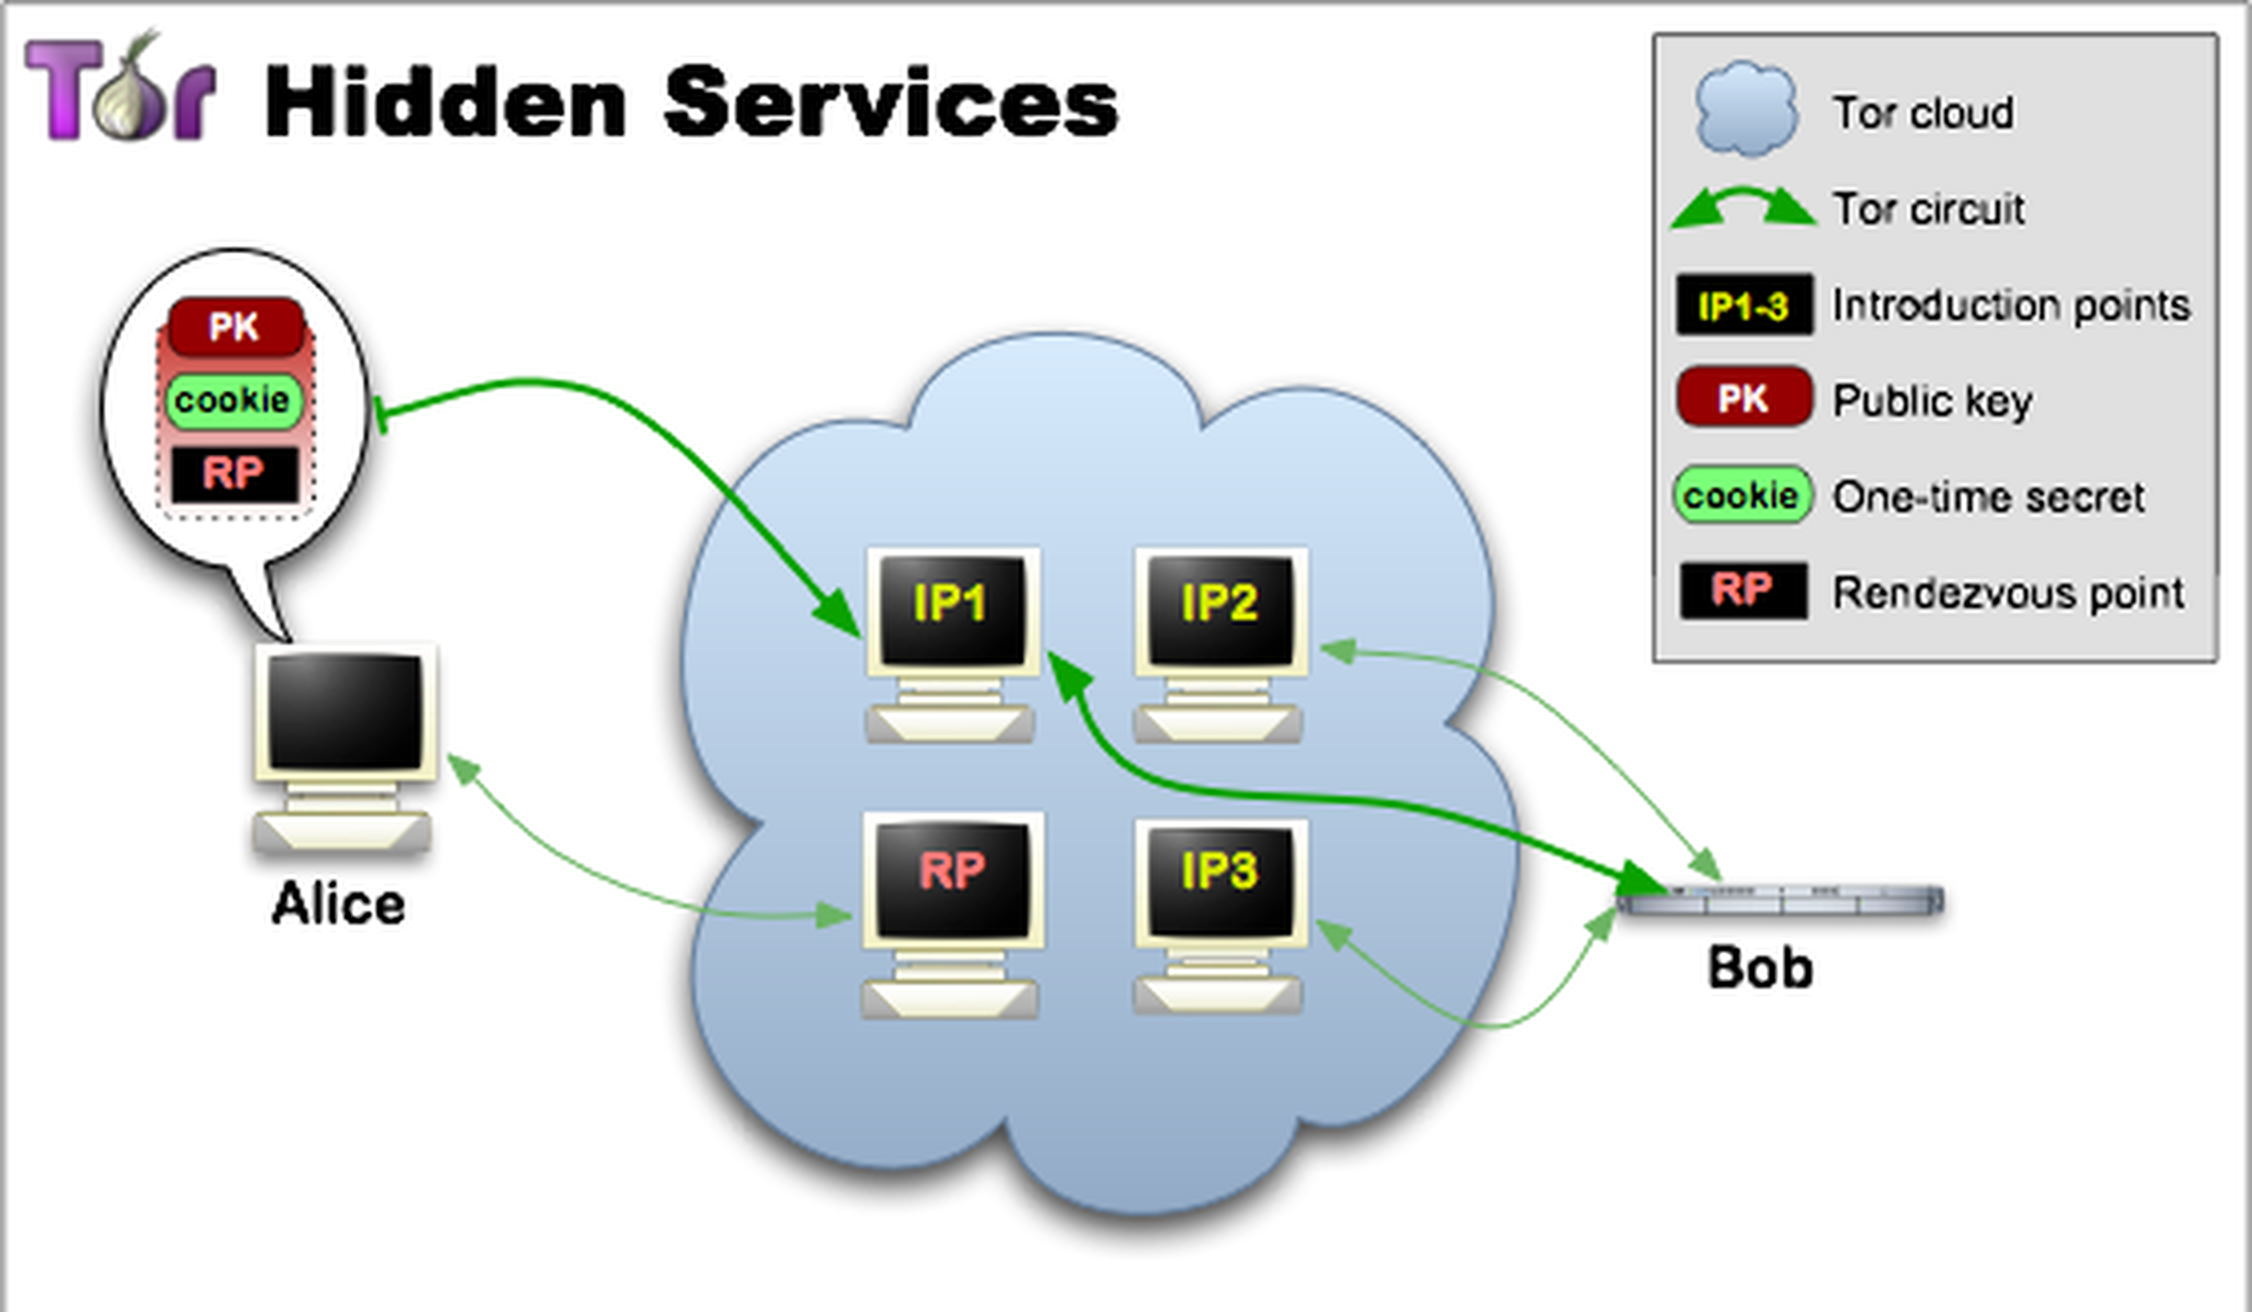
\includegraphics[width=\textwidth]{images/Tor/tor-hidden-service-4-higher.png}
		\caption{Alice uses the encrypted cookie to tell Bob to switch to $ rp $.}
	\end{minipage}
	\hspace{0.5cm}
	\begin{minipage}[b]{0.45\linewidth}
		\centering
		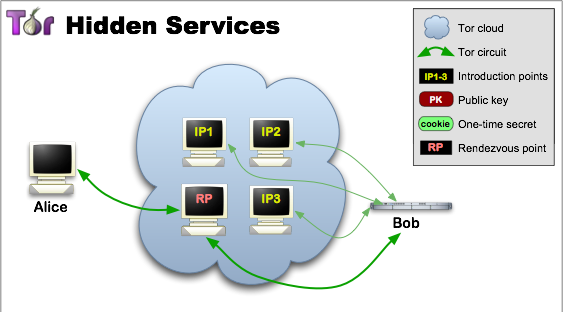
\includegraphics[width=\textwidth]{images/Tor/tor-hidden-service-6.png}
		\caption{Bidirectional communication between Alice and the hidden service.}
	\end{minipage}
\end{figure}

She then sends to $ ip_{1} $ a cookie encrypted with $ B_{K} $, containing $ rp $ and $ sec $. Bob decrypts this message, builds a circuit to $ rp $, and tells it $ sec $, enabling Alice and Bob to communicate. Their communication travels through six Tor nodes: three established by Alice and three by Bob, so both parties remain anonymous. From there traditional HTTP, FTP, SSH, or other protocols can be multiplexed over this new channel.

As of March 2015, Tor hosts approximately 25,000 unique hidden services that together generate around 450 Mbit/s of traffic.\cite{TorMetrics}

% --end rewrite required

\section{Motivation}
\label{sec:Motivation}

As Tor's hidden service addresses are algorithmically derived from the service's public RSA key, there is at best limited capacity to select a human-meaningful name. Some hidden service operators have attempted to work around this issue by finding an RSA key by brute-force that generates a partially-desirable hidden service address (e.g. ``example0uyw6wgve.onion'') and although some alternative encoding schemes have been proposed, (section \label{sec:EncodingSchemes}) the problem generally remains. The usability of hidden services is severely challenged by the non-intuitive and unmemorable base58-encoded domain name. For example, 3g2upl4pq6kufc4m.onion is the address for the DuckDuckGo search engine, \\ suw74isz7wqzpmgu.onion is a WikiLeaks mirror, and 33y6fjyhs3phzfjj.onion and \\ vbmwh445kf3fs2v4.onion are both SecureDrop instances for anonymous document submission. These addresses maintain strong privacy as the strong association between its public key and its address significantly breaks the association between the service's purpose and its address. However, this privacy comes at a cost: it is impossible to classify or label a hidden service's purpose in advance, a fact well known within Tor hidden service communities. Over time, third-party directories -- both on the Clear and Dark Internets -- appeared in attempt to counteract this issue, but these directories must be constantly maintained and furthermore this approach is not convenient nor does it scale well. This suggests the strong need for a more complete and reliable solution.

\section{Contributions}

Our contribution to this problem is five-fold:

\begin{itemize}
	\item We introduce a novel distributed naming system that enables Tor hidden service operators to choose a human-meaningful domain name and construct a strong association between that domain name and their hidden service address.
	\item We rely on the existing Tor network and other infrastructure, rather than introduce a new network. This simplifies our assumptions and reduces our threat model to attack vectors already known and well-understood on the Tor network.
	\item We introduce a novel protocol for proving the non-existence of any domain names.
	\item We enable Tor clients to verify the authenticity of a domain name against its corresponding hidden service address with minimal data transfers and without requiring any additional queries.
	\item We preserve the privacy of both the hidden service and the anonymity of Tor clients connecting to it.
\end{itemize}
